\subsection{Purpose and Procedure}


The objective of this experiment was to measure the wavelength of a red laser beam (\(\lambda\)) using a Michelson interferometer. The laser wavelength was determined by analyzing interference fringes produced by the recombination of two coherent light beams on a screen.  

\begin{figure}[h]
    \centering
    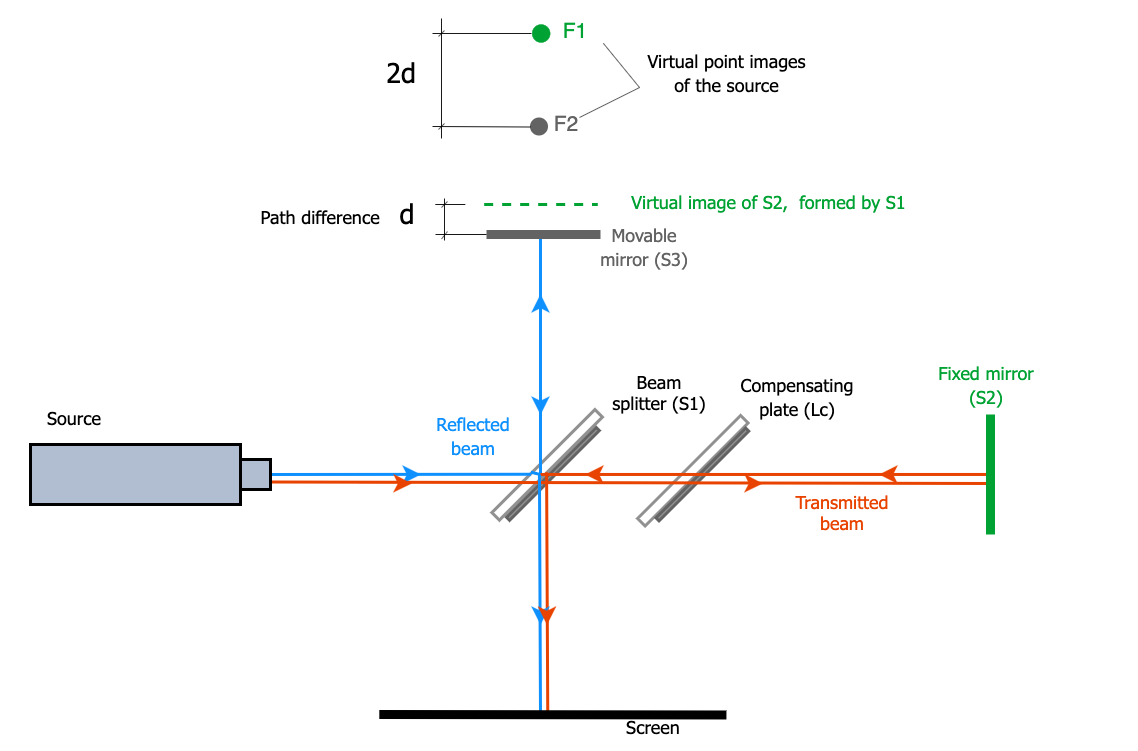
\includegraphics[width=0.9\linewidth]{The_Michelson_interferometer/finalimage1.png}
    \caption{A schematic diagram of the Michelson interferometer}
    \label{fig:michelson}
\end{figure}

The Michelson interferometer consisted of the following key components: Beam Splitter (S1) divides the incident laser beam into two orthogonal paths. Fixed Mirror (S2) reflects one of the split beams. Movable Mirror (S3) adjusted using a micrometer screw to vary the optical path difference. Compensating Plate (Lc) ensures equal optical path lengths for the two beams.  

The beam reflected by S2 traverses S1 once, while the beam reflected by S3 traverses S1 three times. The system creates two virtual coherent point sources (F1 and F2), which produce interference fringes on the screen when their light paths recombine.  

The micrometer screw controlling S3 has a sensitivity of \(2 \, \mu \text{m}\). The displacement of S3 (\(\Delta x\)) was measured as a difference between two micrometer readings, each with an uncertainty of \(2 \, \mu \text{m}\). For the wave calculation, the reflective index \(n_a\) is taken as 1, introducing a negligible error since \(n_a \approx 1.00027\). 
The wavelength was calculated using the formula:  

\[
\lambda = \frac{2 n_a\Delta x}{N} \approx \frac{2 \Delta x}{N}\,
\]  

where \(N\) is the number of fringes observed during the displacement.  

\subsection{Analysis and Error Evaluation}

The measured mirror displacements (\(\Delta x\)), fringe counts (\(N\)), and the calculated wavelengths (\(\lambda\)) are in the table below:  

\begin{table}[!htbp]
    {\par\centering
    \begin{tabular}{cccc}
        \hline
        Measure & $\Delta x \text{ (µm)}$ & $N$ & $\lambda$ \text{(nm)}\\
        \hline
        1   &   42& 130&   646.2\\
        2   &   42& 130&   646.2\\
        3   &   41& 130&   630.8\\
        4   &   40& 130&   615.4\\
        5   &   48& 130&   640.0\\
        \hline
    \end{tabular}
    \par}
    \caption{Measurement of the Wavelength of Laser Light}
\end{table}


The total uncertainty in the wavelength (\(\varepsilon_\lambda\)) arises from uncertainties in the measured displacement (\(\varepsilon_{\Delta x}\)) and the fringe count (\(\varepsilon_N\) = 1). Since \(\Delta x\) is measured as a difference of two micrometer readings, each with an uncertainty of \(2 \, \mu \text{m}\), the total uncertainty in \(\Delta x\) is:  
\[
\varepsilon_{\Delta x} = \sqrt{(2 \, \mu \text{m})^2 + (2 \, \mu \text{m})^2} = 2.83 \, \mu \text{m}
\] \[
\varepsilon_\lambda^2 = \left(\frac{\partial \lambda}{\partial \Delta x} \varepsilon_{\Delta x}\right)^2 + \left(\frac{\partial \lambda}{\partial N} \varepsilon_N\right)^2,
\] where:  \[
\frac{\partial \lambda}{\partial \Delta x} = \frac{2}{N}, \quad \frac{\partial \lambda}{\partial N} = -\frac{2 \Delta x}{N^2}.
\]

The standard deviation of the individual measurements is:  
\[
\sigma = \sqrt{\frac{\sum (\lambda_i - \bar{\lambda})^2}{n-1}} = 13.0 \, \text{nm}
\]  
The standard deviation of the mean is:  
\[
\sigma_{\text{mean}} = \frac{\sigma}{\sqrt{n}} = 5.8 \, \text{nm}
\]  


While the theoretical uncertainty is small, it only accounts for errors in \(\Delta x\) and \(N\), assuming no systematic or random errors. The standard deviation of the mean provides a more realistic estimate, capturing variability between measurements and reflecting the true precision of the experiment.  

The wavelength of the red laser was determined as:  
\[
\lambda = (635.7 \pm 5.8) \, \text{nm}
\]  

This result differs from the nominal 632.8 nm value by about 0.5\%\, indicating good agreement within 1\%\ .

